\documentclass{llncs}
%\usepackage[numbers]{natbib}

%\usepackage{balance}  % for  \balance command ON LAST PAGE  (only there!)
\usepackage[ruled]{algorithm2e}
\usepackage{subfig}
\usepackage{graphicx}
\usepackage{url}
\usepackage{amsmath,amssymb}

\usepackage[colorlinks]{hyperref}

\usepackage{graphicx}				% Use pdf, png, jpg, or eps§ with pdflatex; use eps in DVI mode
								% TeX will automatically convert eps --> pdf in pdflatex

\usepackage{blindtext,graphicx}
\usepackage{multirow}
\usepackage[utf8]{inputenc}
\setlength{\tabcolsep}{13pt}


\begin{document}



\title{SwapMob: Swapping trajectories for mobility anonymization}
\author{Juli\'an Salas\inst{1}%\thanks{With the support of a UOC postdoctoral fellowship}
\and David Meg\'ias\inst{1} \and Vicen\c{c} Torra\inst{2} }
\institute{Internet Interdisciplinary Institute (IN3), Universitat Oberta de Catalunya (UOC), Barcelona, Spain.\\ CYBERCAT-Center for Cybersecurity Research of Catalonia.\\ \email{jsalaspi@uoc.edu, dmegias@uoc.edu, }
\and School of Informatics, University of Sk\"{o}vde, Sk\"{o}vde, Sweden. \\ \email{vtorra@his.se}.
}


\maketitle

\begin{abstract}
%
%Mobility data is a rich and complex resource of patterns, which goes from traffic and congestion trends in a city, to individual movements in closed spaces.
Mobility data mining can improve decision making, from planning transports in metropolitan areas to localizing services in towns.
However, unrestricted access to such data may reveal sensible locations and pose safety risks if the data is associated to a specific moving individual. This is one of the many reasons to consider trajectory anonymization.


Some anonymization methods rely on grouping individual registers on a database and publishing summaries in such a way that individual information is protected inside the group.
Other approaches consist of adding noise, such as differential privacy, in a way that the presence of an individual cannot be inferred from the data.


In this paper, we present a perturbative anonymization method based on swapping segments for trajectory data (SwapMob). It preserves the aggregate information of the spatial database and at the same time, provides anonymity to the individuals.


We have performed tests on a set of  GPS trajectories of 10,357 taxis during the period of Feb. 2 to Feb. 8, 2008, within Beijing.
We show that home addresses and POIs of specific individuals cannot be inferred after anonymizing them with SwapMob, and remark that the aggregate mobility data is preserved without changes, such as the average length of trajectories or the number of cars and their directions on any given zone at a specific time.


\end{abstract}


\subsection{...TO DO*}

Given a probability model, such as Markov chain models, of the data, and a subsequent decision problem (eg. traffic flow prediction from mobility siumlations based on the learnt Markov chain model), we can limit ourselves to data-anonymizing operators that preserve the (minimal) sufficient statistic of the model.

Intuitively speaking, all the information in the data about the parameters of the model are in the sufficient statistic.
Therefore, by anonymizing the data while preserving the sufficient statistics is decision-theoretically optimal, in the sense of maximizing utility from optimal estimates of the parameters in the probability model.

A {\em sanitizer} $\mathcal{S}$ is a map from the data space $\mathbb{D}$ to a sanitized data space $\mathbb{D}'$, i.e., $\mathcal{S}(d): \mathbb{D} \to \mathbb{D}'$.
A sanitizer may or may not preserve the minimimal sufficient statistics in the data.
A {\em sufficient sanitizer} preserve the minimal sufficient statistics.

... then we can choose between them based only on privacy concerns.


- This is my interpretation of the notes from last day :

We consider probabilistic models for a database $D$ and statistical inference by time homogeneous discrete time Markov Chains with probability matrix $P$ and rate matrix $Q$ which is a sufficient statistic of $D$ for this model

- Rigth now I could generate the probability matrices with states $S_i$ as spatial points with rounded coordinates (coarsened locations), it is quite straightforward, and they still represent square areas in the map.

- Prove that SwapMob preserves the minimal sufficient statistic

- Argue why other methods would not preserve the minimal sufficient statistic

- Explain synthetic generation of trajectories

For future work:

- Calculating privacy and utility may be left as future work.



- Where are these used in transportation (some citations and brief explanations)

\subsection{\bf Marina>  SHORTEN and ADD to Intro, still work in progress}


Origin Destination Matrices (ODM) comprise an important base for transportation modelling as way to depict travel demand. OD trip generation models serve as basis for transport planning, construction, performance assessment, and as such have potential to affect regional economies. ODM are utilised in transportation studies as part of trip generation modelling, representing estimated traffic flows.

ODM of $m$ Origins $i$ and $n$ Destinations $j$ is a matrix of size $(m+1) \times (n+1)$ containing flow values $T_{ij}$, such as number or share of trips from $i$ to $j$ \cite{Rodrigue2009}. The row $(i+1)$ contains total arrivals to destination $j$ from all origins, the column $(j+1)$ contains total departures from origin $i$ to all destinations, and the bottom right element contains the total flows in the model $T_{i+1,j+1} = \sum_{j=1}^n \sum_{i=1}^m T_{i,j}$ \cite{EVANS1970} (see for example \ref{table:ODMeg}).

\begin{table}[]
\caption{Example Origin Destination Matrix from a spatial interaction survey}
\centering

\begin{tabular}{cl ccc r}
\noalign{\smallskip}
\noalign{\smallskip}
											& 							& \multicolumn{3}{c}{Destinations $j$}  	&  \\ [0.5ex]
											&  					 	&  Uppsala     & Stockholm    & Arlanda    & $\bf \sum T_i$ \\ [1.3ex]
%\cline{2-6}
\multirow{3}{*}{\rotatebox[origin=c]{90}{Origins $i$}} & Uppsala          & 2000          & 5            & 20        & \bf{2025} \\
                             & Stockholm        & 10            & 100          & 10        & \bf{120}  \\
                             & Arlanda          & 20            & 5            & 0         & \bf{25}   \\  [1.3ex]
%\cline{2-6}
\noalign{\smallskip}
\multicolumn{1}{l}{}         &  $\bf \sum T_j$      & \bf{2030} & \bf{110} & \bf{30} & 2170
\end{tabular}
\label{table:ODMeg} % is used to refer this table in the text
\end{table}

{\bf rephrase the stuff below, a bit repetitive}

ODM [implicit] parameters include: cut-off departure time from Origins, cut-off arrival time to Destinations, mode of transportation, spatial aggregation level for Origins ({\it e.g.} by TAZ - Traffic Analysis Zones, ZIP code areas, square grid, {\it etc.}), spatial aggregation levels for Destinations. Spatial aggregation of O and D data by zones can provide zone measurements and disaggregation by links can provide link based counts. In other words, keeping overall ODM counts but not keeping the trajectory data in between can be used as input to traditional traffic allocation models. Keeping link flows but not keeping the OD for each trajectory enables to calibrate flows within these models.

Estimating OD demand is an important input into traffic assignment models, used to plan infrastructure and access performance. Traffic flows can be estimated using OD demand matrix, infrastructure network capacity and traffic controls. And later using sensor observations of density and travel time, these modelled flows can be compared to the observed traffic ODM to derive performance measures. Moreover, disaggregated OD matrices (by hour or more generally by 1 time unit) can be used to calibrate traffic assignment models to predict flows through specific links.


This means that aggregated ODM is good for total demand estimation, but disaggregated ODM are useful for observing flows in the network links and comparing those to the output flows from traffic allocation models.

ODM are constructed based on estimations from travel studies: field, online and telephone traffic surveys, traffic volume counts \cite{robillard1975},  check-point intercept interviews, license plate and other video analyses, {\it etc}. Automatically generated data (e.g. CDR \cite{iqbal2014}) are increasingly used as a base for constructing ODM, reducing survey costs and improving accuracy of route choice estimations. All of these methods yield an incomplete matrix, so often Spatial Interaction Models \cite{WILSON1967} are used to estimate the complete ODM.






\section{Introduction}

With the pervasive use of smartphones and the location techniques such as GPS, GSM and RFID, the opportunities to deliver content depending on current user location have increased.
Location Based Services (LBS) provide considerable advantages such as allowing users to benefit from live
location-based information for transportation, recommendations of places of interest, or even the opportunity to meet friends in nearby locations.
Such location-based data can be useful also for intelligent transportation systems, in which vehicles may serve as sensors for collecting information about traffic jams, weather, and road conditions.


However, revealing users' locations may have some privacy risks. If the data is linked to the real identities it may reveal personal preferences (e.g., sexual, political or religious orientation), or it may be used for inferring habits and know the time when a person is at home or away.
To avoid such inconveniences, a variety of anonymization techniques have been developed to hide the identity of the user or her exact location, e.g, \cite{Terrovitis:2011}.


Moreover, as Giannotti et al. mention in \cite{Giannotti2012}, big data (in particular trajectory data) may be used  to understand human behavior through the discovery of individual social profiles, by the analysis of collective behaviors, spreading epidemics, social contagion, and to study the evolution of sentiment and opinion; however, trusted networks and privacy-aware social mining must be pursued and methods for protection and anonymization for such data must be developed to enforce the data subjects' rights and promote their participation.

\section{Related work}
Different solutions have been proposed for anonymizing trajectories in data publishing. Abul et al. \cite{Abul2008}, propose the $(k, \delta)$-anonymity model, which consists on publishing a cylindrical volume of radius $\delta$ that contains the trajectory of at least k moving objects. Note that this idea is an extension of the concept of $k$-anonymity for databases \cite{Samarati:1998}.


Terrovitis and Mamoulis \cite{Terrovitis:2008} consider a discrete spatial domain, e.g., spatial information is given in terms of addresses in a city map.
Hence, the user trajectories are expressed as sequences of POIs.
They present the use case of the RFID cards from the Octopus\footnote{http://www.octopuscards.com/} company in Hong Kong, which collects the transaction history of its customers. The company may want to publish sequences of transactions by the same person as trajectories, for extracting movement and behavioral patterns. However, if a given user, Alice, uses her card to pay at different convenience stores that belong to the same chain (e.g., convenience stores), that company may reidentify Alice if her sequence of purchases is unique in the published trajectory database.


A similar approach in \cite{Pensa2008} is obtained by transforming sequences by adding, deleting, or substituting some points of the trajectory, while preserving also frequent sequential patterns \cite{Agrawal:1995} obtained by mining the anonymized data.


In \cite{Hoh2005} and \cite{Hoh06}, Hoh et al. discuss the use of mobility data for transportation planning and traffic monitoring applications to provide drivers with feedback on road and traffic conditions.
For modelling the threats to privacy in such datasets, they assume that an adversary does not have information about which subset of samples belongs to a single user, however by using multi-target tracking algorithms \cite{Reid79analgorithm} subsequent location samples may be linked to an individual that is periodically reporting his anonymized location information.

In \cite{Hoh06} they consider the attack of deducing home locations of users by leveraging clustering heuristics used together with the decrease of speed reported by GPS sensors. Then, propose data suppression techniques by changing the sampling rate (e.g, from 1 minute to 2,4 and 10) for protecting from such inferences.

In \cite{Hoh2005}, in order to prevent adversaries from tracking complete individual paths, they propose an algorithm that perturbs slightly the trajectories of different individuals (to make them closer) in such a way that the adversary may not be able to follow which segment of the path corresponds to which user by using multi-target tracking algorithms.
This is done with a constraint on the Quality of Service, which is expressed as the mean location error between the actual and the observed locations. They argue that adequate levels of privacy can only be obtained if the density of users is sufficiently high.


This is closely related to \cite{Beresford2003} in which Mix Zones are introduced, these are spatial areas on which users' location is not accessible, hence when users are simultaneously present on a mix zone, their pseudonyms are changed. This procedure is performed to difficult the linkage of the incoming and outgoing path segments to the same specific user.

They design a model for location privacy protection that aims to preserve the advantages of location aware services while hiding their identities from the applications that receive the users' locations.
The existence of a trusted middleware system (or sensing infrastructure) is assumed and the applications register their interest in a geographic space with the middleware, such space is called application zone. Examples of such application zones are hospitals, universities or supermarket complexes, in general it could be any open or closed space.

The regions in which applications cannot trace user movements are called mix zones, and the borders between a mix zone and an application zone are called boundary lines.
Applications do not receive traceable user identities, they receive pseudonyms that allow communication between them. Such communication passes through the trusted intermediary and the pseudonyms of users change when they enter a mixed zone.


In order to measure location privacy, Beresford and Stajano \cite{Beresford04mixzones} define the anonymity set as the group of people visiting the mix zone during the same time period. However, as the boundary and time when a user exits a mix zone is strongly correlated to the boundary and time when the user enters it, such information may be exploited by an attacker, therefore they use the information theoretic metric that Serjantov and Danezis \cite{Serjantov2002} proposed for anonymous communications which considers the varying probabilities of users sending and receiving messages through a network of mix nodes.


This is modeled in \cite{Beresford04mixzones} as a movement matrix in which they record the frequency of ingress and egress points to the mix zone at several times.
Then, a bipartite weighted graph is defined in which vertices model ingress and egress pseudonyms and edge weights
model the probability that two pseudonyms represent the same underlying person. Therefore, a maximal cost perfect matching of these graphs represents the most probable mapping among incoming and outgoing pseudonyms.

However, since the solution to many restricted matching problems (such as this one) is NP-hard \cite{Tanimoto1978}, Beresford and Stajano \cite{Beresford04mixzones} describe a method for achieving partial solutions.


An approach that does not consider middleware to obtain location privacy is proposed in Chapter 9 from \cite{Gidofalvi2007}. It consists of a system with an untrusted server and clients communicating in a P2P network for privacy preserving trajectory collection.
The aim of their data collection solution is to preserve anonymity in any set of data being stored, transmitted or
collected in the system. This is achieved by means of $k$-anonymization and swapping.
Briefly, the protocol consists of the clients recording their private trajectories, cloaking them among $k$ similar trajectories and exchanging parts of those trajectories with other clients in the P2P network. However, the final step (the data reporting stage) clients send anonymous partial trajectories to the server, that have been generated in such a way that the server can filter all the synthetic trajectory data that has been generated for cloaking during the process, and recover the original trajectory.

One of the advantages of performing trajectory anonymization on the user side, as in \cite{Romero-Tris2016}, is that the anonymization process is no longer centralized. Thus data subjects gain control, transparency and more security for their data.

%\subsection{Differential privacy approaches}

For a brief overview of privacy protection techniques and a discussion of $k$-anoymity and differential privacy models in different frameworks, cf. \cite{Salas:2018}.


In \cite{Chen:2012}, a differential privacy model for transit data publication is considered, using data from the Soci\'{e}t\'{e} de Transport de Montr\'{e}al (STM). The data are modeled as sequential data in a prefix tree that represents all the sequences by grouping the sequences with the same prefix into the same branch.
Their algorithm takes a raw sequential dataset $D$, a privacy budget $\epsilon$, a user specified height of the prefix tree $h$ and a location taxonomy tree $T$, and returns a sanitized dataset $\tilde{\mathcal{D}}$ satisfying $\epsilon$-differential privacy.
For measuring utility, in the STM case, sanitized data are mainly used to perform two
data mining tasks, count query and frequent sequential pattern mining \cite{Agrawal:1995}.


Other $\epsilon$-differentially private mechanism for publishing trajectories called SDD (Sampling Distance and Direction) can be found in \cite{Jiang:2013}.
They focus on ship trajectories with known starting point and terminal point.
And consider that two trajectories $T$ and $T'$ with the same number of positions are adjacent if they differ at exactly one position excluding the starting point and the terminal point.


In \cite{Xiao:2015}, a differentially private algorithm for location privacy is proposed, following a discussion on the (in)applicability of differential privacy in a variety of settings, such as \cite{Chatzik:2013} and  \cite{Kifer:2011}.
Their algorithm considers temporal correlations modeled as a Markov chain and proposes the ``$\delta$-location set'' to include all probable locations (where the user might appear). The authors argue that, to protect the true location, it is enough to “hide” it in the $\delta$-location set in which any pairs of locations are not distinguishable.
However, they leave the problem of protecting the entire trace of released locations as future work.


In this paper, we present an anonymization method considering that the data are dynamic, the rate at which the information is collected is not constant, and the databases are being generated as the data is received.
%online and in real time with a database that is updating constantly.


\section{Proposed method: SwapMob}

We propose a method for anonymization of mobility data by swapping trajectories, which works in a similar way as the mix zones but in a non-restricted space.


Our algorithm (SwapMob) simulates an online P2P system for exchanging segments of trajectories. That is, when two users are near they interchange their partial trajectories, see section \ref{sec:cross}.
In this way, all users' trajectories are mixed incrementally, and the moving users keep generating segments of trajectories that are being swapped. In the end, each trajectory retrieved is made of small segments of trajectories of different individuals, who have met during the day, as depicted in Figure \ref{fig:swap}. Hence, the relation between data subjects and their data is obfuscated while keeping a precise aggregated data, such as the number of users in each place at each time and the locations that have been visited by different anonymous users.

We formalize our method after a brief explanation of previous definitions and assumptions.

\subsection{Definitions}
We assume that we have a database in which the $i$-th observation is a tuple ($ID_i$, lat$_i$, long$_i$, $t_i$) that
consists of the individual's identifier ($ID_i$), the latitude (lat$_i$), longitude (long$_i$) and timestamp ($t_i$).

Then, the trajectory $T_x$ of an individual \texttt{$x$} will consist of all the observations with identifier \texttt{$x$} ordered by their timestamps \texttt{$t_i$}.
These can be represented as $T_x = (x_1, x_2, \ldots, x_m)$ if there are $m$ observations for individual $x$.


We say that \emph{two individuals meet} or their trajectories cross (on points $x_i$ and $y_j$) if they have been co-located. We denote this by $x_i \approx y_j$. Note that being co-located depends on thresholds for proximity ($\chi$) and time ($\tau$), since the sampling rate of positions is not regular nor constant. Moreover two persons cannot be in the exact same place at the same time.

We define a \emph{matching} as a maximal subset of pairs of elements of a set.

We denote by $Sw(T)$ the resulting trajectory after all swaps have been applied to $T$.
Next, we define the following two primitives for our algorithm: \emph{generate random matching} and \emph{swap}.
\begin{enumerate}

\item \emph{Swap:}
Given two trajectories $T_x = (x_1, \ldots, x_i, x_{i+1}, \ldots)$ and \linebreak
$T_y= (y_1, \ldots, y_j, y_{j+1}, \ldots)$ that meet in points $x_i$ and $y_j$, a swap of $T_x$ with $T_y$ at points $x_i$ and $y_j$ results in $Sw(T_x) = (y_1, \ldots, y_j, x_{i+1}, \ldots)$ and
\linebreak
$Sw(T_y)= (x_1, \ldots, x_i, y_{j+1}, \ldots)$.
\item \emph{Generate random matching:}

Given a set of elements $S = s_1, s_2,\ldots, s_m$, we generate a random matching by making pairs of the first $m/2$ with the following $m/2$ numbers, followed by a random permutation of all numbers $m$.
\end{enumerate}

Note that, in case that the number of elements $m$ is odd, to generate a matching we must leave out one element and that all possible random matchings can be generated following our procedure.

\subsubsection{Crossing paths and Swapping} \label{sec:cross}
We propose a model such that two peers get in contact (meet) if they have been co-located on a similar timestamp depending on parameters of proximity $\chi$ and time $\tau$.


Next, we simulate SwapMob protocol by swapping the users IDs when the users have passed close enough.
We calculate the set of users that get in contact in a given time interval, and choose a random matching among them when they are even and a matching of all but one, when they are odd.
Here, the swapping is carried out in a pairwise manner, but it could be done as a permutation such as in \cite{Beresford04mixzones}.

Note that changing pseudonyms (IDs) is equivalent to swapping the partial trajectories.


\begin{figure*}[!t]
	\center{
	\subfloat[\scriptsize Original trajectories] {
		  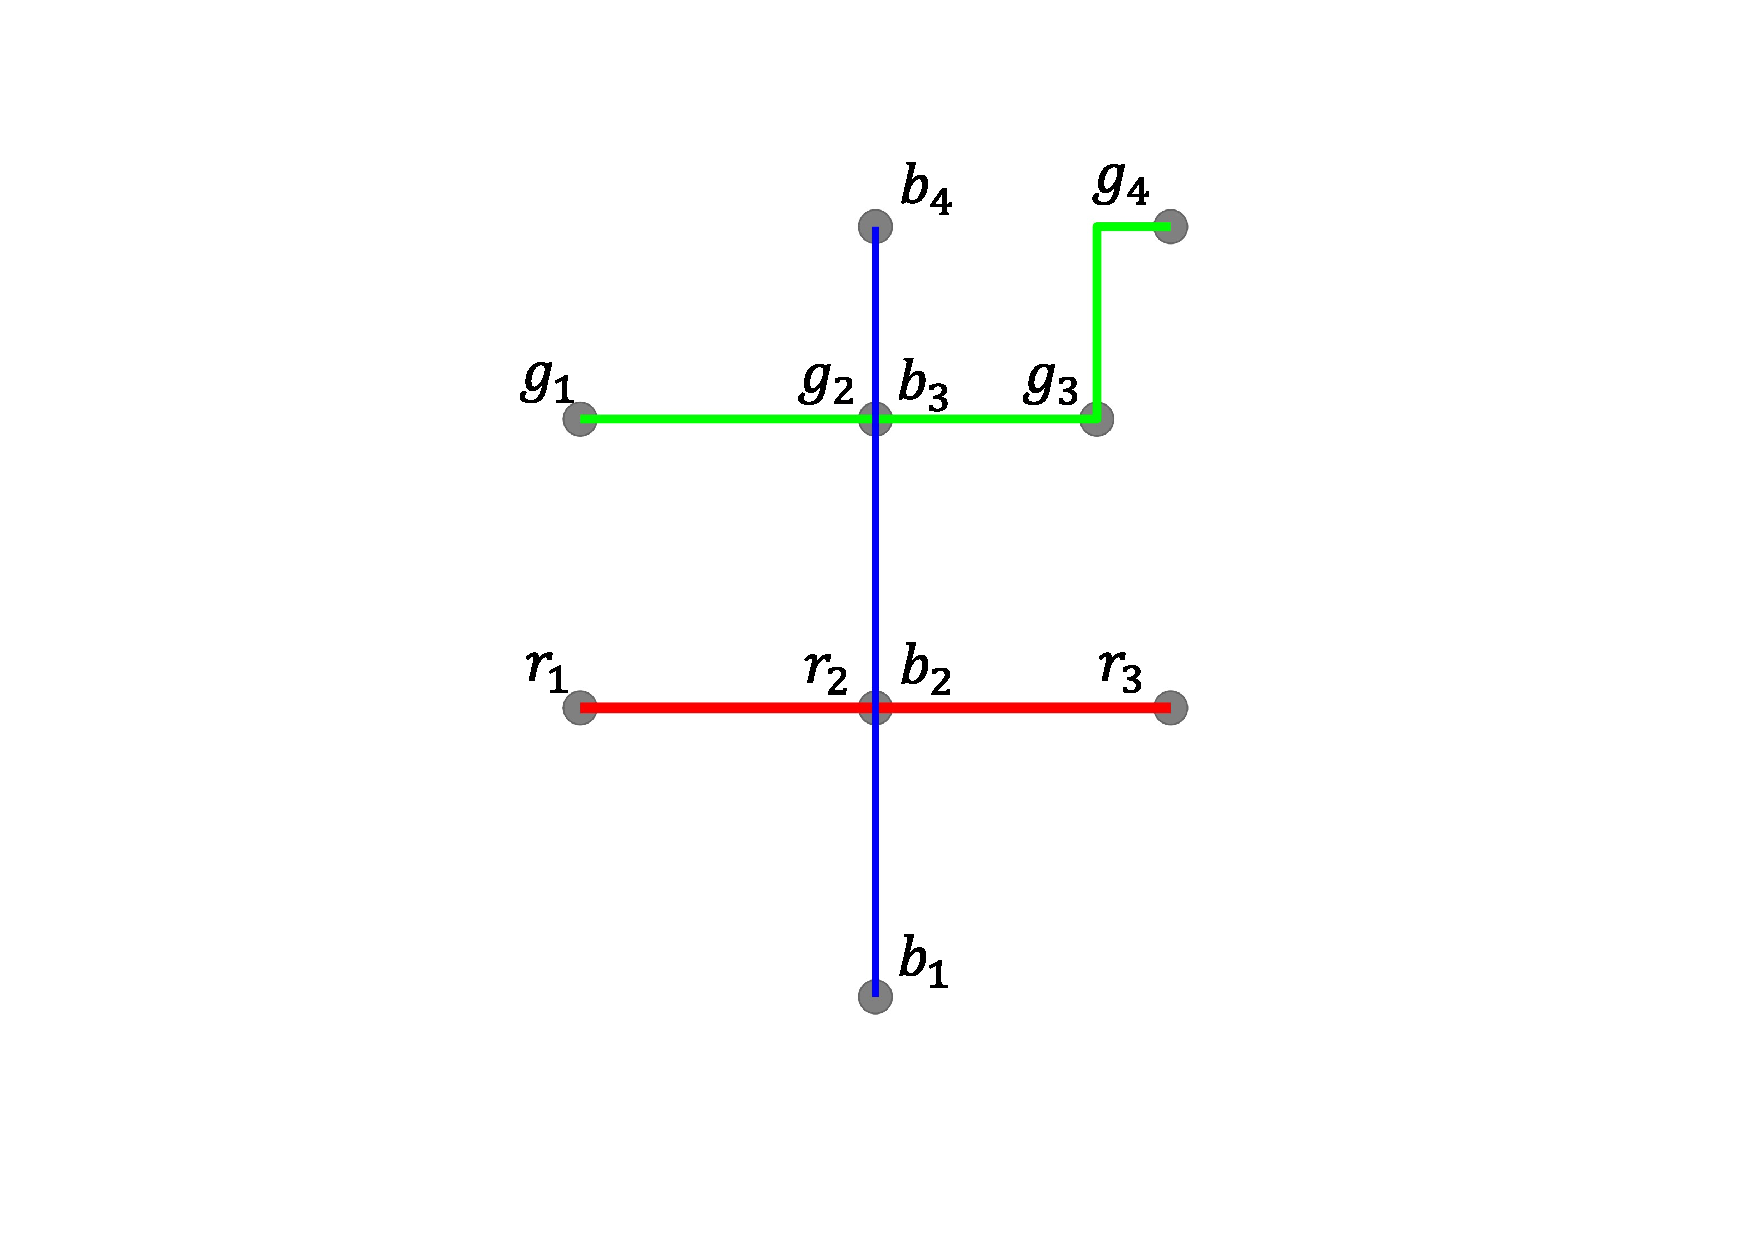
\includegraphics[width=0.34\textwidth]{figures/cross1.pdf}
    }
	\subfloat[\scriptsize After first swap]{
				  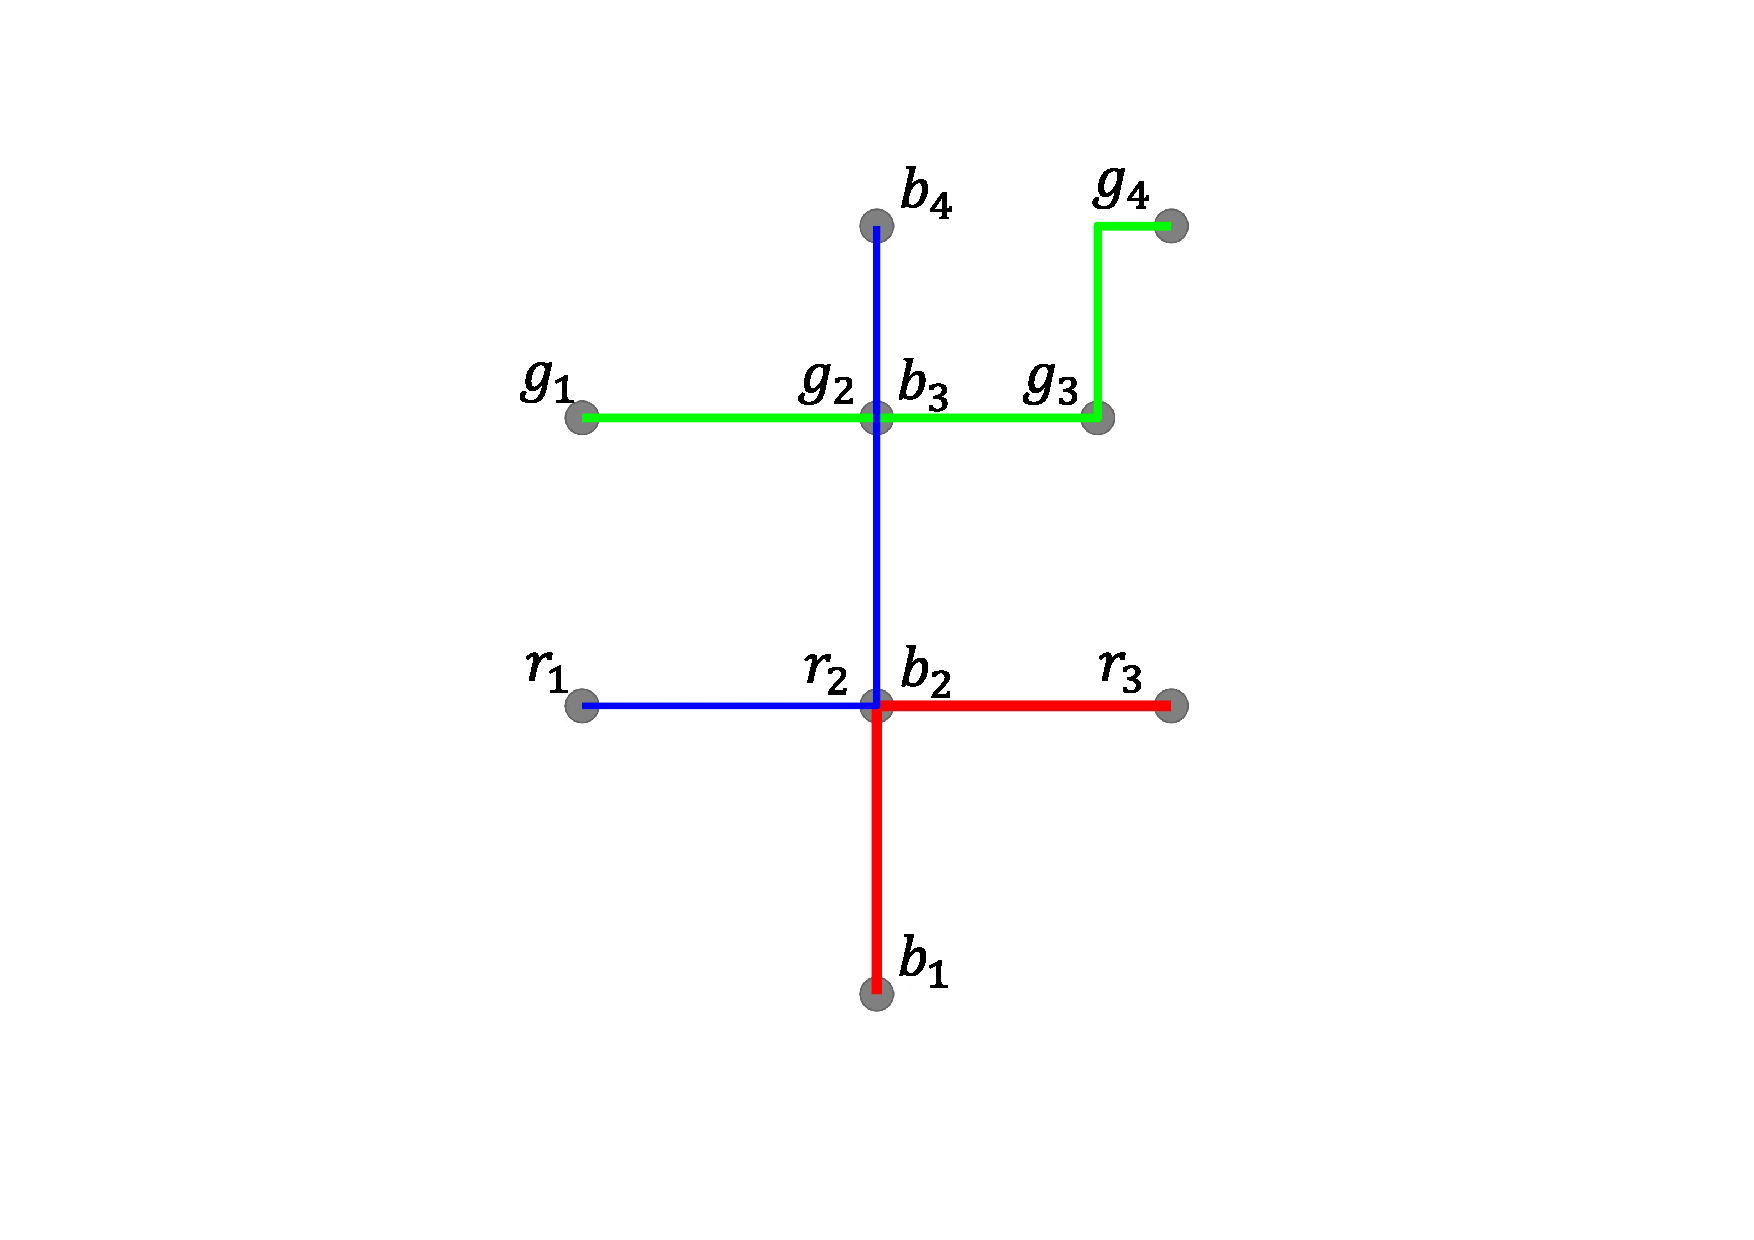
\includegraphics[width=0.34\textwidth]{figures/cross2.pdf}
   	}
    \subfloat[\scriptsize After second swap] {
				  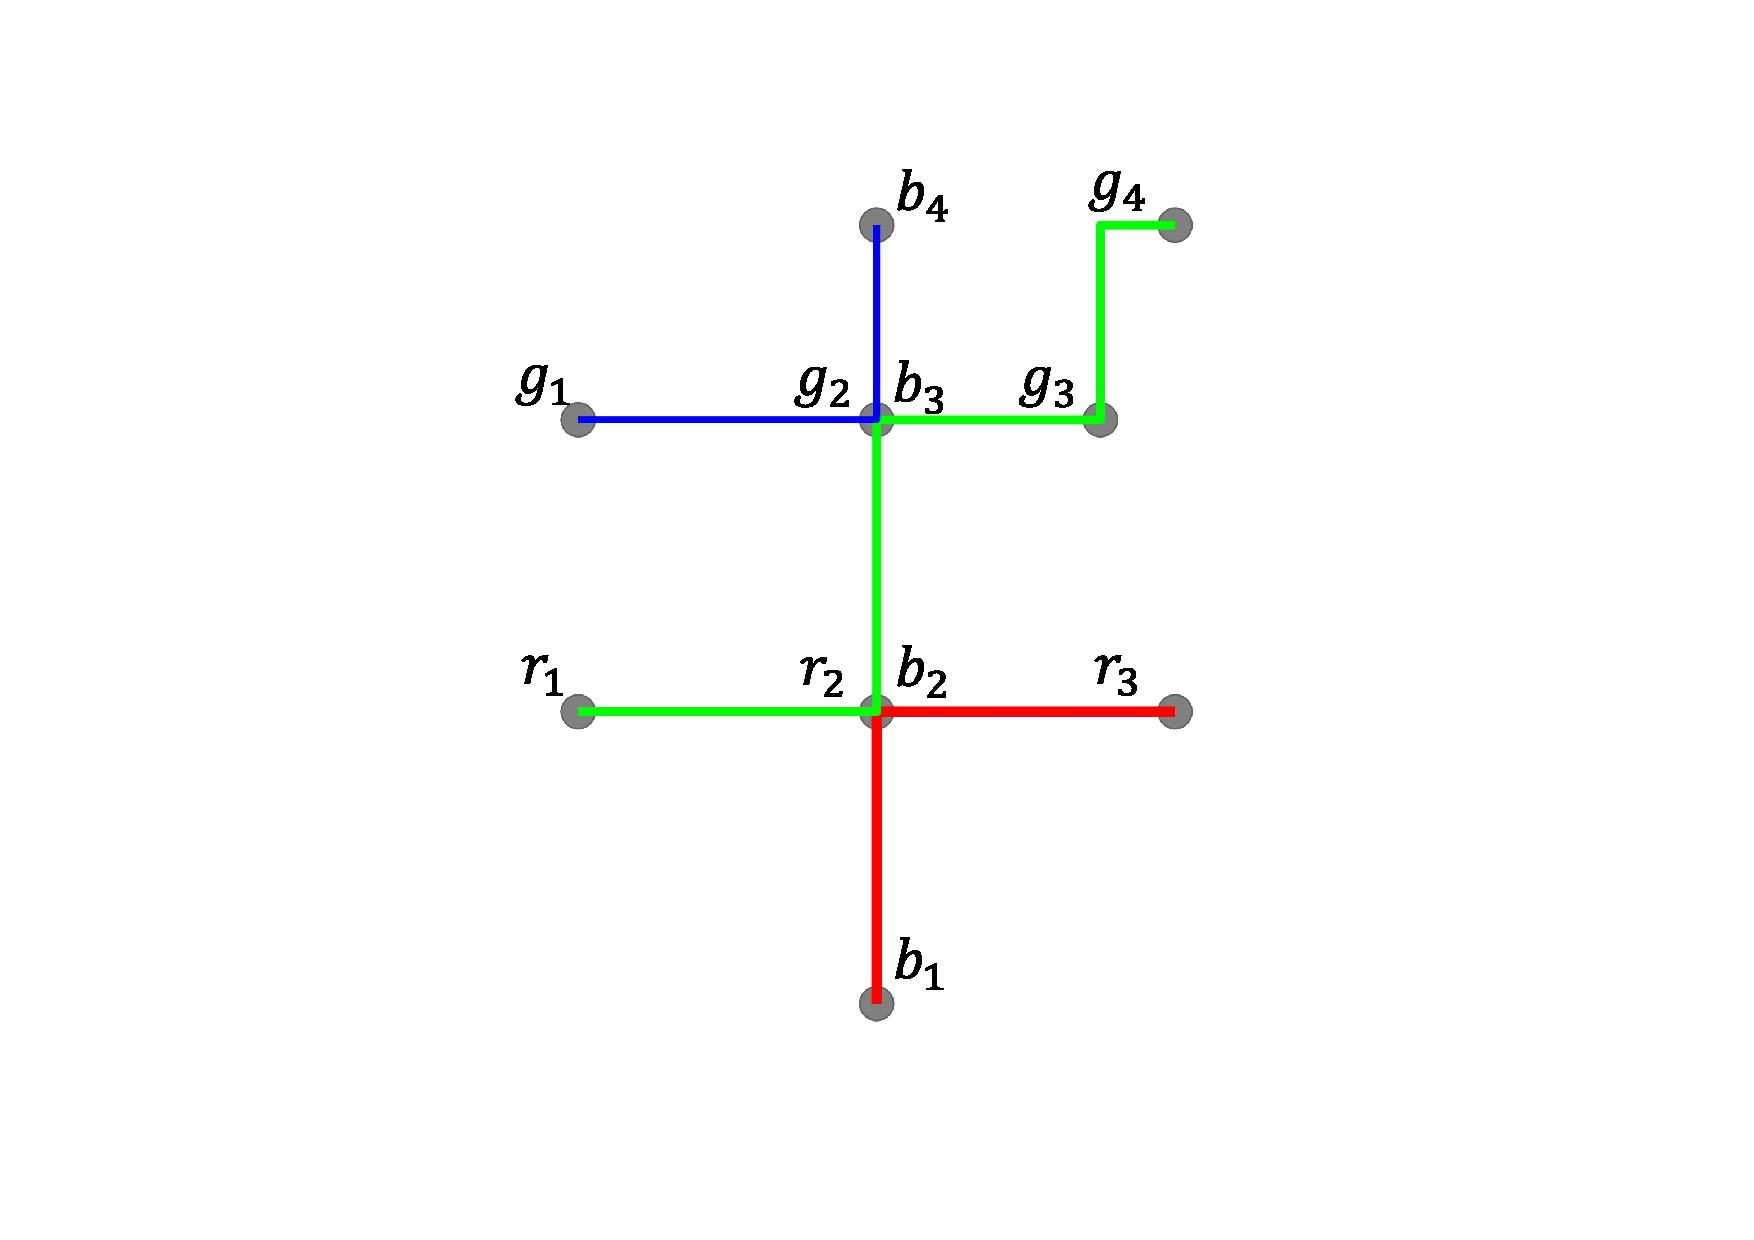
\includegraphics[width=0.34\textwidth]{figures/cross3.pdf}
   	}
\caption{Three trajectories before and after swapping}
\label{fig:swap}
}
\end{figure*}


In Figure \ref{fig:swap}, we present an example of three simple trajectories crossing $T_r, T_g, T_b$. We assume that they are moving from left to right and upwards, $T_r = (r_1, r_2, r_3)$, $T_g = (g_1, g_2, g_3, g_4)$ and $T_b = (b_1, b_2, b_3, b_4)$. Note that we are also assuming that the blue trajectory meets the red trajectory first ($b_2 \approx r_2$) and then the green trajectory ($b_3 \approx g_2$). In this tiny example, we can see how the iterative swaps preserve parts of the trajectory intact, but at the end each trajectory has parts of many others, such as the green one which ends having a segment of the blue trajectory, a segment of the red and a segment of its original trajectory $Sw(T_g)=(r_1, r_2, b_3, g_3, g_4)$.


\begin{algorithm}[t]
\SetAlgoNoLine
\KwIn{Trajectory Database. Thresholds for time $\tau$ and proximity $\chi$. }
\KwOut{Swapped trajectories identifiers $Sw(T_i)$.}

Partition the timestamps $t =\bigcup \tau_j$ in intervals of length $\tau$

\For{each pair of registers $i,j$ in interval $\tau_j$}{
  \If{ $dist(l_i, l_j)< \chi$}{
    add $i,j$ to close records list (possible swaps) $S_{\tau_j}$ at the given time interval.
  }
}
generate random matching with possible swaps in $S_{\tau_j}$\

order all swaps in $\bigcup S_{\tau_j}$ by timestamp\

\For{each pair $i\approx j$ in $\bigcup S_{\tau_j}$}
{swap $T_i$ with $T_j$}
\KwRet {Swapped trajectories $Sw(T_i)$}

\caption{Offline algorithm for swapping trajectories}
\label{alg:one}
\end{algorithm}


\subsection{SwapMob anonymizer}

We follow a similar architecture to the one in \cite{Hoh06} in which a Trusted Third Party ($TTP$) knows the
vehicles identities but can not access sensor information (such as position and  speed); and a Service Provider ($SP$) knows the sensor measures but not the identities.
Further, the $SP$ calculates which records are close to each other without knowing to which individual they belong and communicates them to the $TTP$ (in this case SwapMob anonymizer) such that it can swap their identities without knowing at which location they were.

This is achieved in the following way (See Figure \ref{fig:protocol}):
\begin{enumerate}
\item Users communicate with SwapMob, sending their sensor data ($M$) encrypted with the public key ($K_{SP}$) of $SP$. SwapMob keeps the number of register ($i$), which user has sent it ($u_i$), its current pseudonym ($ID_i$), the timestamp ($t_i$) and the encrypted sensor data $E(M_i, K_{SP})$, which includes their encrypted location ($l_i$).

\item SwapMob sends the vector ($i, t_i, E(M_i, K_{SP}))$ to the $SP$, who decrypts $E(M_i, K_{SP})$ and keeps a buffer of data on interval $\tau_j$ that contains all timestamps between timestamp $t_j$ and $t_{j+1}$ and has length $\tau$, that is $\tau_j =\{ t : t_j < t < t_{j+1}\}$.

\item $SP$ sends the set $S_{\tau_j}$ of registers that were at distance less than the predefined threshold $\chi$ during the interval of time $\tau_j$ back to SwapMob, more formally $S_{\tau_j} = \{ i,i' : d(l_i, l_{i'}) < \chi \mbox{ and } t_i,t_{i'} \in \tau_j\}$. SwapMob calculates the swaps and stores the users and swapped $IDs$ list,
that is, for every record $i$ SwapMob keeps the corresponding swapped id $Sw(ID_i)$ and the user ($u_i$) to which such pseudonym corresponds.

\item Finally, every given period of time which could  be daily, weekly or monthly, SwapMob reports the list  of ($i, Sw(ID_i)$) to $SP$.
%In our example, it is reported each 24 hours at 18:05.

\end{enumerate}
The authentication data integrity of the communications can be guaranteed with a hash-based message authentication code.


\begin{figure*}
\center{
  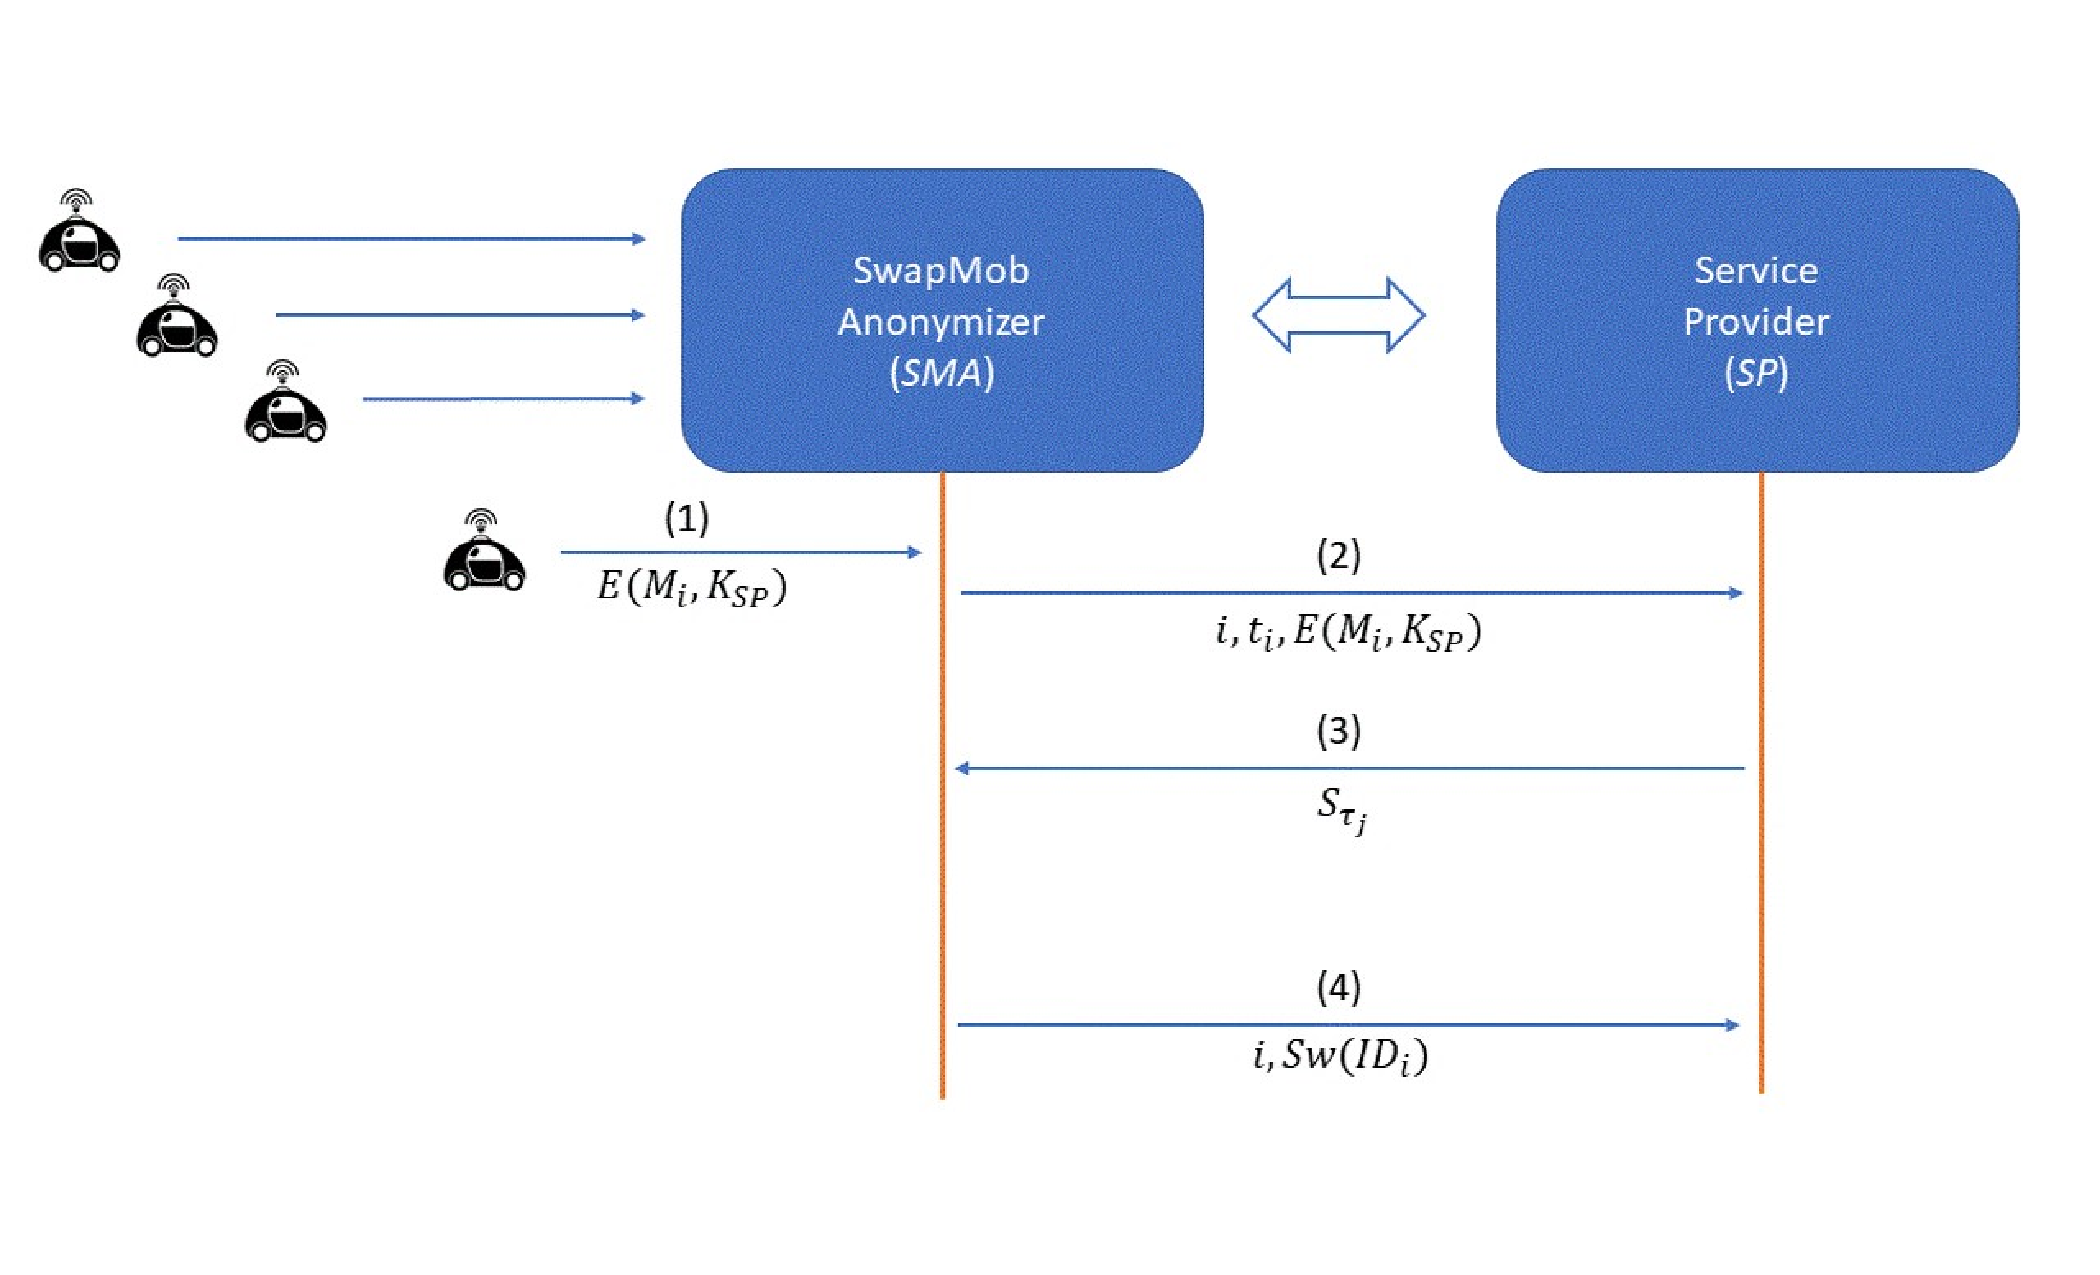
\includegraphics[width=0.95\textwidth]{figures/Protocol6.pdf}
  \caption{Architecture of our system}
  \label{fig:protocol}
}
\end{figure*}

In this way, $SP$ obtains the measures of all sensors $M$ in real-time (Step 2), and at the end of the day also gets the anonymized trajectories of the users that generated them (Step 4).
Even, though $SP$ knows which records belong to $S_{\tau_j}$ (Step 3), $SP$ does not know to which other record they have been swapped during period $\tau_j$, and by the iterative swappings it gets even harder to associate them to a specific user.

At the same time, SwapMob only knows the users, the timestamps at which they have crossed, and the reported trajectories are already anonymized by SwapMob (Step 4).

Our system, can be applied for the use case proposed in \cite{Beresford2003}, by defining a set of swap zones (similar to the mix zones) and adding the restriction that the swapping cannot be performed outside such places. Then, the spatio-temporal trajectories of users between such swap zones could be monitored in an anonymous and precise way.


However, there will still be some differences. Namely, the swap zone that we consider is the entire application zone, whereas in \cite{Beresford2003} a user entering a mix zone can be distinguished from another user emerging from the same zone if the size of the mix zone is too large.

This same argument justifies that the distance and time parameters, $\chi$ and $\tau$ must not be too large either in our algorithm, otherwise swapping could not be credible.



\subsection{Protecting against reidentification} % by Home/Work location
It is well known that de-identification does not necessarily means anonymization. The same attributes that are used for extracting knowledge, may be used for pointing to a specific individual, and uniquely relating his/her data to her real identity.

Other notions of privacy are defined depending on the context, which may be of statistical databases \cite{Danezis15}, networks \cite{Zhou:2008}, or geo-located data.

By identifying the POIs of an individual, it is possible to infer his habits (e.g., does sport, travels a lot), the locations that he visits frequently (may be related to political or religious beliefs) or even related to health (clinics, hospitals). This may also be used to infer his schedule, predict his future locations,  and learn his past locations and possibly his personal relations by observing frequent or periodic co-location.
Moreover, such habits and locations can be easily used to reidentify the individuals behind the data. As it has been proven on previous anonymity studies on anonymity of home/work location.

Regarding this topic, Golle and Partridge studied in \cite{Golle:2009} workers who revealed their home and work location with noise or rounding on the order of a city block, a kilometer or tens of kilometers (census block, census tract, or county) and showed that the sizes of the anonymity set were respectively 1, 21 and 34,980. That is, when the data granularity was on the order of a census block, the individuals were uniquely identifiable, and for granularities on the order of census track or county, they were protected within sets of size 21 or 34,980.
In \cite{Zang:2011},  Zang and Bolot inferred the top $N$ locations of a user from call records and correlated such information with publicly-available side  information such as census data.  Then, they showed that the top 2 locations likely correspond to home and work location and that the anonymity sets are drastically reduced if an attacker infers them.


Therefore, for protecting the individuals against reidentification, is crucial to protect their home addresses and POIs, to provide them with minimum guarantees of keeping them anonymous.
Swapped data may not allow for following a specific individual and his whereabouts, and thus, this will not permit personalization or individual classification, which are ways of protecting their privacy.


A different approach regarding the possibility of reidentification and the (im)possibility of protection, is in \cite{demontjoye2013}, where they measure the uniqueness of human mobility traces depending on their resolution and the available outside information, assuming that an adversary knows $p$ random spatio-temporal points. Then, they coarsen such data spatially and temporally to find a formula for uniqueness depending on such parameters.


We argue that SwapMob preserves anonymity by dissociating the segments of trajectories from the subject that generated them.

An attacker may know several spatio-temporal points of an individual that uniquely identify him. However, to link a register in the anonymized database to such an individual, the points known by the attacker must belong to the same trajectory after swapping. In most cases, the attacker will not learn the entire trajectory information since the published trajectory is made of segments from many different individuals.
Of course, when publishing the trajectories, it should be noted that they have been generated by SwapMob, and the anonymization may be reversed if the SwapMob Anonymizer and the Service Provider (see Figure \ref{fig:protocol}) share their information for guaranteeing accountability.



\subsection{Utility of swapped data}\label{sect:util}
In this paper we are assuming that the interest of using data anonymized by SwapMob is for making mobility maps and predictions that may be useful for intelligent transportation systems and for planning in a city.
As Hoh and Gruteser proposed in \cite{Hoh2005}, pre-specified vehicles could periodically send their locations, speeds, road temperatures, windshield wiper status and other information to the traffic monitoring facility. These statistics can provide information on the traffic jams, average travel time or the quality of specific roads, and can be used for traffic light scheduling and road design.

Furthermore, the sensors do not necessarily have to be attached to vehicles, they could be carried on mobile phones, and the utility of using the individuals for sensing is preserved, since all their sensor data, including all their movements and timestamps (in aggregate) are kept intact by SwapMob.


In \cite{Calabrese2011}, a real-time urban monitoring platform and its application to the City of Rome was presented, they used
a wireless sensor network to acquire real-time traffic noise from different spots, GPS traces of locations from 43 taxis and 7268 buses, and voice and data traffic served by each of the base transceiver stations from a telecom company in the urban area of Rome. These are few examples of sensor that could be carried by individuals, anonymized and transmitted to a service provider via SwapMob.


Another example is the offline mining in \cite{Yuan2011} representing the knowledge from taxi-drivers as a landmark graph could be done with SwapMob anonymized data. A landmark is defined as a road segment that has been frequently traversed by taxis, and a directed edge connecting two landmarks represents the frequent transition of taxis between the two landmarks. This graph is then used for traffic prediction and for providing a personalized routing service.


In general, lossless maps of flows in the city can be obtained by using SwapMob at several aggregation levels and for different timestamps.



\section{Empirical evaluation}
We tested our algorithm on the T-drive dataset
\cite{Yuan2010},\cite{Yuan2011} which contains the GPS trajectories of
10,357 taxis during the period of Feb. 2 to Feb. 8, 2008 within
Beijing. The total number of points in this dataset is about 15
million and the total distance of the trajectories reaches to 9
million kilometers. It is important to note that not all taxis appear
every day and not all report their positions at the same interval. The
average sampling interval is about 177 seconds and 623 meters. Each
measurement contains the following data: taxi id, date time,
longitude, latitude.

\subsection{Applying SwapMob on the data}
Before applying SwapMob to the dataset we perform some cleaning of the
data. We begin by removing all measurements for which the latitude and
longitude is outside the box $[115, 117] \times [39, 41]$, these
measurements are far outside Beijing and most of them have both
latitude and longitude equal to zero, which indicates that the
measurement is most likely not valid. We then remove all trajectories
which have no measurements belonging to them at all. Doing this
removes 756561 invalid measurements and 77 trajectories that have no
measurements, we end up with 10280 trajectories and 16906423
measurements.

For applying SwapMob we consider two taxis co-located if they are in
the same square of width 0.001 degrees ($\chi = 0.001$), about 111
meters, in the same minute ($\tau = 60$). Note that this is about 6
and 3 times less the average sampling interval for distance and time
in the dataset.

With this we get that the number of possible swaps between all the
trajectories is 641262. The average number of swaps for each
trajectory is 137. Of all the 10280 trajectories 9508, 92\%, take part
in at least 20 swaps, for the 772 trajectories with less than 20 swaps
we have the distribution seen in Figure \ref{fig:swaps-distribution}.
We see that 324 trajectories don't participate in any swaps at all,
however 265 of these trajectories have less than 10 measurements
(compared to an average of more than 1000).

We can conclude that most of the trajectories participate in several
swaps, only a small amount participate in less than 20 swaps and that
most of the trajectories that don't participate in any swap have very
few measurements.

\begin{figure}
  \center
  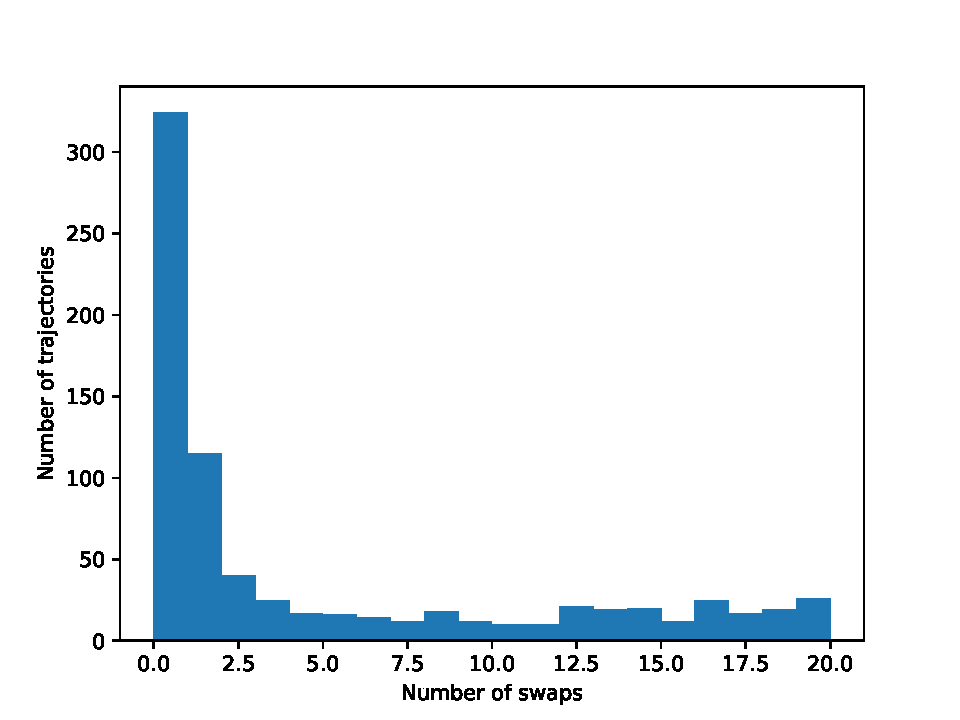
\includegraphics[width=0.5\textwidth]{figures/swaps-distribution.pdf}
  \caption{Frequency histogram of number of swaps for trajectories for
    the 772 trajectories participating in less than 20 swaps.}
  \label{fig:swaps-distribution}
\end{figure}

\subsection{Reidentification by linkage}
\label{sec:reidentification}
In this section we simulate an adversary who knows exact locations and
timestamps, and tries to reidentify a trajectory in the dataset. In
\cite{demontjoye2013} a similar kind of adversary is considered, but
in that case it only knows location and timestamp up to some
resolution, in contrast to this our adversary should be considered to
be very strong. We discuss how the swapped trajectories could be
de-anonymized using this kind of information and show that in most
cases only a small fraction of the full trajectory is disclosed.

Since we assume the adversary knows exact locations and timestamps it
can identify an (unswapped) trajectory using only one such point,
assuming no two measurements are exactly the same. After applying
SwapMob the adversary can still identify trajectory with the
measurement, but it doesn't know exactly which parts of the trajectory
have been swapped and thus doesn't learn the full trajectory. It does
however learn part of the trajectory, it can follow the trajectory
from the known measurement forward in time until the next swap can
occur and also backwards in time until the previous swap that could
occur. This part of the trajectory is known to belong to the wanted
individual, since no swaps were performed on it, but after the swaps
the adversary doesn't know for certain which path belongs to the
original trajectory.

To measure how much the adversary learns we thus have to look at how
long the segments between the swaps are. Since every trajectory
participate in an average of 137 swaps and is thus split into an
average of 138 segments. Knowing one point the adversary will learn
one of these segments. To see how much the adversary learns we can
thus look at how long these segments are. For each trajectory we can
look at the longest such segment and compare its length to that of the
whole trajectory. Doing this and plotting the empirical cumulative
distribution function for it we get the plot in Figure
\ref{fig:ECDF-max-part}. With length we here mean the number of
measurements, but elapsed time and distance traveled would both be
other natural choices for the length.

Figure \ref{fig:ECDF-max-part} shows that for more than 75\% of all
trajectories the longest unswapped segment makes up less than 20\% of
the total trajectory. For 90\% of the trajectories the number is less
than 40\%. For most trajectories an adversary will thus learn only a
small fraction of the original trajectory.

We can also consider the case when the adversary knows several points
of the trajectory. If the extra points lie on the same segment of the
trajectory as the first one no more knowledge is gained. However, if
the extra points lie on other segments of the trajectory the adversary
learns also these and more of the trajectory is disclosed. If the
adversary knows several segments of the trajectory it can also try to
infer which way was taken between them, that way learning more than
just the disclosed segments. Analysing this is however outside the
scope of this article and left as further research.

\begin{figure}
  \center
  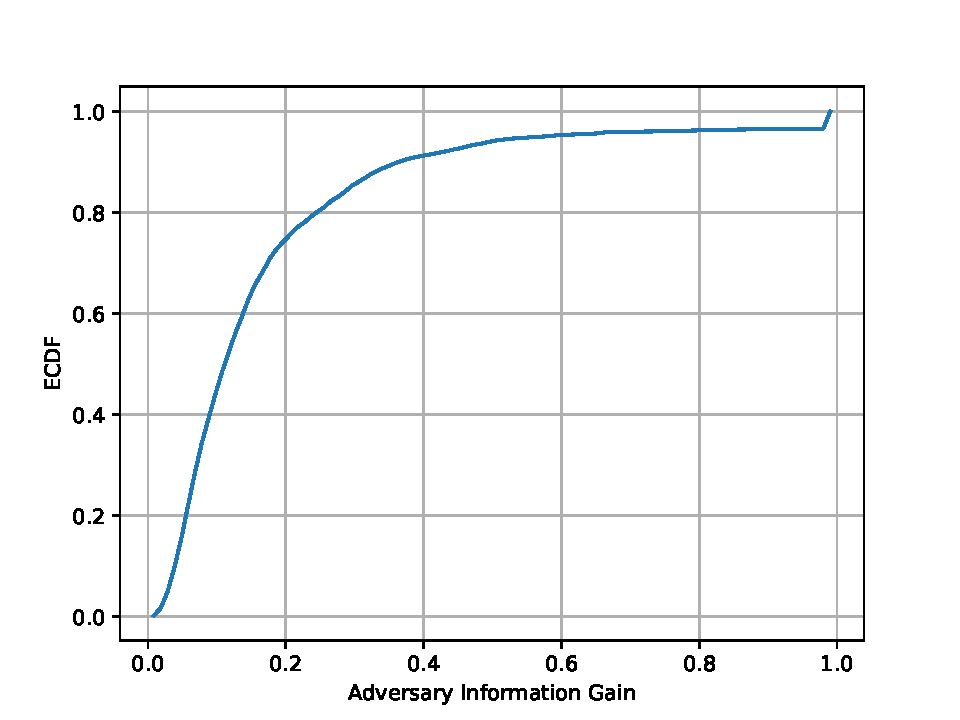
\includegraphics[width=0.5\textwidth]{figures/ECDF-max-part.pdf}
  \caption{Length of the longest unswapped segment as percentages of
    the total length for each trajectory. The length was here given by
    the number of measurements.}
  \label{fig:ECDF-max-part}
\end{figure}

\subsection{Privacy when preserving the ODM}
We now look at what happens with the privacy measures when we restrict
swapping to preserve the ODM, introduced in Section \ref{sec:ODM}. The
data is precisely the same as before but now, for two trajectories to
swap they have to start and end in the same destination, this is in
addition to the earlier requirements for allowing a swap.

We define the destinations used in the ODM by a grid, we partition the
city into a grid of equally sized squares. Bigger squares give a
coarser grid and smaller squares a finer grid. How coarse the grid is
will be given by the width of the squares in degrees (latitude and
longitude), a lower width then corresponds to a finer grid. Starting
location for a trajectory will be given by the square that its first
measurement belongs to and end location by the square that its last
measurement belongs to. In general it might be more appropriate to
have start and end location to be determined by the location of the
trajectory at a certain time of the day. However, for keeping it
simple, we choose to use only the first and last measurement.

We'll look at how the preserved privacy change when we go from having
no grid to having a very coarse grid and then making it finer and
finer.

In Figure \ref{fig:num-swaps-OD} we see how the number of possible
swaps change when we make the grid finer. At first we have the number
of swaps without a grid and then we have the numbers for grids of
squares of the given width. The largest width used is 1 degree, about
11100 meters, which can be compared to the distance of 0.001 degrees,
about 111 meters, that we used for determining if two trajectories
were close. It splits the city into four parts, of which two contains
most of the measurements. The smallest width is 0.01 degrees, about
1110 meters, which is then 10 times the length used for determining
proximity.

We see that the number of possible swaps quickly decrease as the grid
gets finer. Even at the coarsest grid the number of swaps is halved
compared to having no grid. When the grid width goes below 0.1 we have
very few possible swaps.

Since the preserved privacy heavily depends on the number of possible
swaps we expect it to quickly decrease as the grid becomes finer. We
can confirm this by computing the same measurement as in Section
\ref{sec:reidentification} for each grid size, see Figure
\ref{fig:ECDF-max-part-OD}. The line corresponding to having no grid
is the same as in Figure \ref{fig:ECDF-max-part} and we can see that
the privacy decreases as the grid becomes finer.

We can conclude that the preserved privacy is greatly influenced by
the grid size of the ODM. If the grid is to fine almost no swaps occur
and the SwapMob algorithm is not efficient. For very coarse grids the
privacy is still reduced but could depending on the application still
be considered acceptable.

\begin{figure}
  \subfloat[\scriptsize The number of possible swaps depending on the
  grid size. Going from having no grid to a very fine grid.] {
    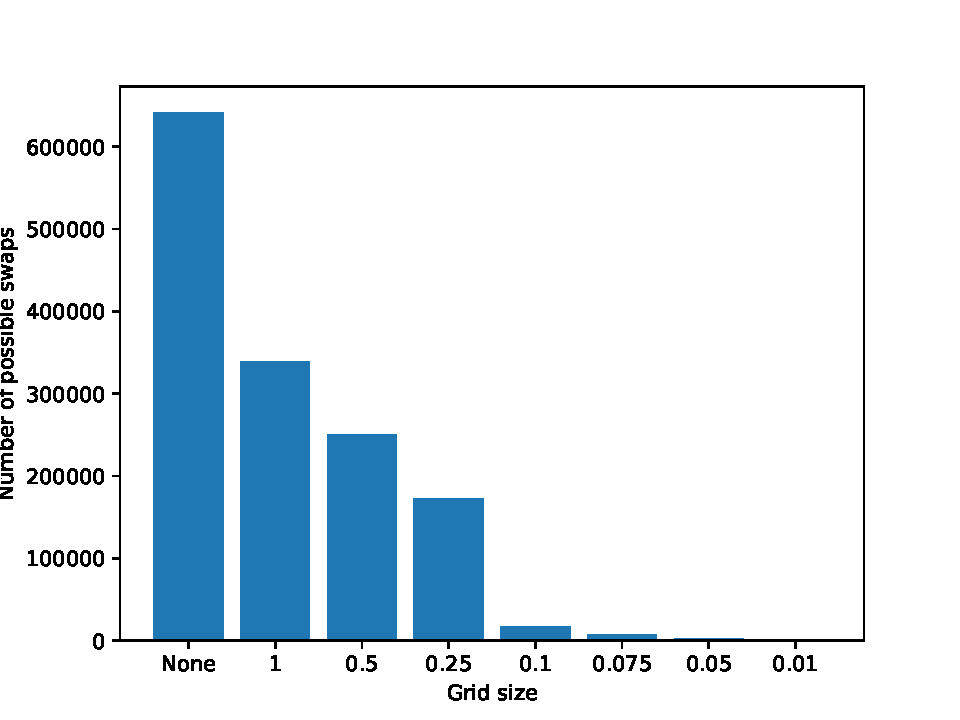
\includegraphics[width=0.5\textwidth]{figures/num-swaps-OD.pdf}
    \label{fig:num-swaps-OD}
  }
  \hfil
  \subfloat[\scriptsize Length of the longest unswapped segment as
  percentages of the total length for each trajectory for different grid
  sizes. The length of the trajectory was here given by the number of
  measurements.] {
    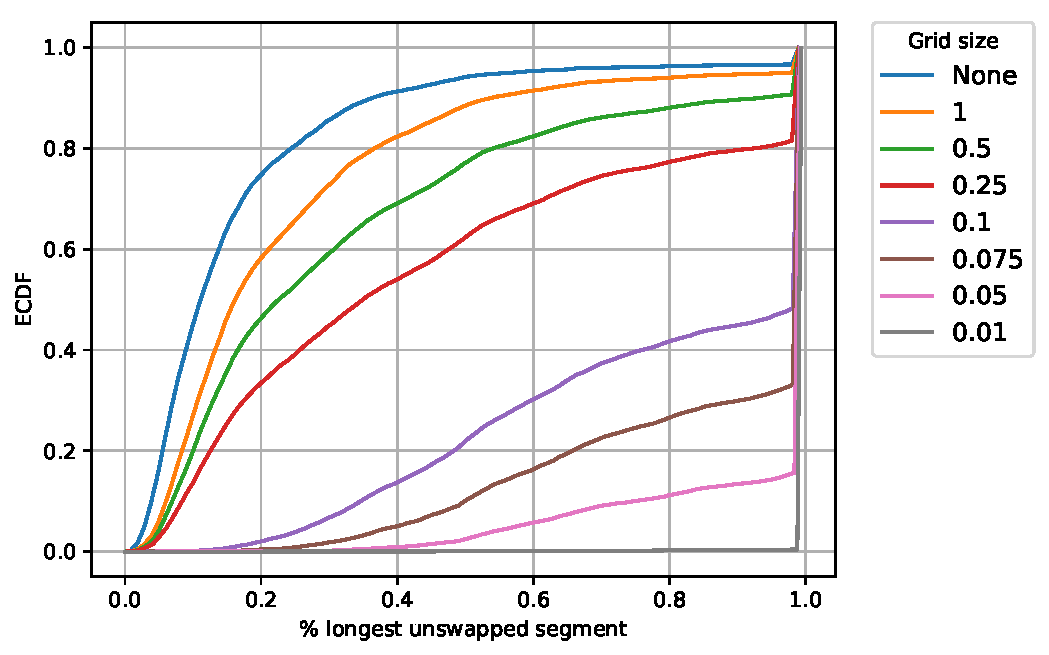
\includegraphics[width=0.5\textwidth]{figures/ECDF-max-part-OD.pdf}
    \label{fig:ECDF-max-part-OD}
  }
  \caption{Preserved privacy when also preserving the ODM}
  \label{fig:OD}
\end{figure}

\section{Conclusions}

We have defined and tested a novel algorithm for real-time mobility data \linebreak
anonymization that consists on swapping trajectory segments. In contrast to the $k$-anonymity or differential privacy models for trajectory anonymization, the proposed method does not modify the data, but its association to specific individuals, and it is performed on real time, without the need of having the entire dataset.
The proposed protocol tackles both identity and location privacy,
 and our data model can be adapted to protect either single trajectory positions, as they lose the relation to the individual who has generated the data, or the whole trajectories, since they are mixed among many different peers.

We show that is not possible to infer correctly the home locations after the anonymization and, also, that an adversary who knows exact points of the trajectory is not able to use them for reidentification, because in most cases they no longer correspond to the anonymized trajectory. And, even in the improbable case that the adversary correctly relates the anonymized trajectory with the original, we have shown that he cannot infer the entire trajectory but just a small part of it.


We have simulated our protocol with an offline algorithm, although, the protocol could be run in real time in which data is transmitted by user devices to our anonymizer that communicates and collaborates with a server. By changing the anonymizer for a group protocol, the protocol could provide security against collusion between the service provider and the anonymizer.
%
%In this paper, we considered that the SwapMob anonymizer is used for intelligent transportation systems, however, it could also anonymize different sensor data in addition to car sensors, such as smartphones or any mobile device, it could even be used for anonymizing transactions, and any other types of trajectory data.
%

It must be pointed out that swapping cannot be carried out when an individual does not cross anyone in her path. Hence, the proposed technique will not anonymize the individuals who do not cross anyone in their daily activity.
%This will depend on the period on which the trajectory information is retrieved by the server from SwapMob.
However, it is not very common for an individual to spend too much time without meeting someone or going out from home. Moreover, such individuals can be kept outside the database without compromising its utility.
The use case considered is for obtaining aggregate mobility data and exact count queries, which neither $k$-anonymity or differential privacy can provide.

Nevertheless, this comes at the cost of modifying the trajectories and possibly losing individual trajectory mining utility.
Future work directions to solve this issue are to add the restriction of non-swapping streets or non-swapping zones for improving the utility to better preserve entire trajectories inside a given street or zone.

\section*{Acknowledgments}
Juli\'{a}n Salas acknowledges the support of a UOC postdoctoral fellowship.
This work is partly funded by the Spanish Government through grant TIN2014-57364-C2-2-R ``SMARTGLACIS'', and Swedish VR (project VR 2016-03346).

\bibliographystyle{splncs03}
%\bibliographystyle{IEEEtran}%
\bibliography{biblio-swap}




\end{document}
